\documentclass[12pt]{ai_conquer2026}
\addbibresource{references.bib}
\title{%
  \begin{center}
        \Large {AI VIET NAM -- AI Conquer 2026}\\[.5ex]  
        \Huge \textbf{A Comparative Study of Tree-based Models for Healthcare Risk Prediction: Cross-validation and SHAP-based Stability Analysis}\\[.5ex]
  \end{center}
}


\posttitle{
\author{
\begin{minipage}{\textwidth}
\centering
{
\vspace{-1.5em}
Group \textbf{Numby}
\\[1cm]
\begin{tabular}{p{6cm}p{5cm}p{3cm}}
    \textbf{Name} & \textbf{Position} & \textbf{Role} \\
    Le Quang Thanh & Tech Leader & Team Leader\\
    Nguyen Van Vi & AI Engineer (Pipeline) & Member\\
    Le Thanh Lam & AI Engineer (Data) & Member\\
    Pham Minh Dang Tran & AI Engineer (Model) & Member\\
    Tan Du & QA / Reviewer & Member
\end{tabular}
\\[1cm]
}\
\end{minipage}
}
}
\date{}

\pagestyle{fancy}
\fancyhf{}
\lhead{\href{https://www.facebook.com/aivietnam.edu.vn}{\textcolor{aivnGreen}{\bfseries AI VIET NAM (AI Conquer 2026)}}}
\rhead{\href{https://aivietnam.edu.vn/}{\textcolor{aivnGreen}{\bfseries aivietnam.edu.vn}}}
\fancyfoot[C]{\thepage}
\renewcommand{\headrulewidth}{1.0pt}
\renewcommand{\headrule}{{\color{aivnGreen}\hrule width\headwidth height\headrulewidth \vskip-\headrulewidth}}

\begin{document}
\maketitle
\vspace{-5.5em}
\setlength{\epigraphwidth}{0.6\textwidth}

\section{Research Summary}
\label{sec:research_summary}

\newpage
\setcounter{tocdepth}{2}
\tableofcontents
% \listoftables
% \listoffigures
\thispagestyle{fancy}

\newpage

\section{Introduction and Research Questions}
\label{sec:introduction}

\subsection{Research Context}

Healthcare risk prediction has become an important application of machine learning,
particularly with the increasing availability of structured healthcare data. Machine
learning models can be used to identify patterns in demographic, clinical, and
physiological features and estimate the risk of developing a disease or experiencing
an adverse health outcome. Such predictive models may provide useful
decision-support information for healthcare-related analysis.

Among machine learning approaches for structured data, tree-based models are
widely used because they can capture nonlinear relationships and feature
interactions while requiring relatively few assumptions about the underlying data
distribution. In particular, boosting-based models such as AdaBoost, XGBoost,
and LightGBM have demonstrated strong predictive capabilities and are commonly
applied to classification problems.

However, healthcare datasets can differ substantially in terms of sample size,
feature distributions, missing values, and class imbalance. As a result, the
performance of a particular model may vary across datasets. Evaluating multiple
models across multiple healthcare datasets under a consistent experimental
protocol can therefore provide a more comprehensive understanding of their
behavior.


\subsection{Research Problem}

Although tree-based models can achieve strong predictive performance,
comparing models based solely on a single train-test split or a single performance
metric may provide an incomplete view of their reliability. A model that performs
well on one particular split may exhibit considerable variation when trained on
different subsets of the data.

Cross-validation provides a systematic approach for evaluating this variability by
repeatedly training and evaluating models on different data partitions. Therefore,
model comparison should consider not only average predictive performance but
also the consistency of performance across cross-validation folds.

Furthermore, predictive performance does not indicate why a model produces its
predictions. In healthcare-related machine learning, identifying influential
features can provide additional insight into model behavior. SHapley Additive
exPlanations (SHAP) can be used to quantify the contribution of individual
features to model predictions. However, feature importance obtained from a
single training run may not necessarily remain consistent when the training data
changes.

This raises a second stability concern: whether the explanations produced by a
model remain consistent across different cross-validation folds. A feature that
appears highly important in one fold but substantially decreases in importance
in other folds may indicate that the corresponding interpretation is sensitive to
the training data.

Therefore, this study considers both predictive stability and explanation
stability when comparing tree-based models for healthcare risk prediction.


\subsection{Research Questions}

Based on the research problem described above, this study investigates the
following research questions:

\begin{itemize}
    \item \textbf{RQ1:} How do AdaBoost, XGBoost, and LightGBM compare in
    healthcare risk prediction across multiple datasets?

    \item \textbf{RQ2:} How stable is the predictive performance of these models
    across cross-validation folds?

    \item \textbf{RQ3:} How stable are SHAP-based feature importance rankings
    across cross-validation folds?
\end{itemize}


\subsection{Contributions}

This study makes the following contributions:

\begin{itemize}
    \item \textbf{Systematic comparison of boosting-based tree models.}
    We provide a controlled empirical comparison of AdaBoost, XGBoost, and
    LightGBM for healthcare risk prediction across multiple datasets using a
    consistent experimental protocol.

    \item \textbf{Evaluation of predictive stability.}
    In addition to reporting predictive performance, we analyze the variability
    of model performance across cross-validation folds to assess the
    consistency of the models.

    \item \textbf{Analysis of SHAP explanation stability.}
    We investigate the stability of SHAP-based feature importance rankings
    across cross-validation folds, providing an empirical assessment of
    whether model explanations remain consistent under different training
    subsets.

    \item \textbf{Multi-dataset evaluation.}
    By evaluating the models across multiple healthcare datasets, the study
    examines whether observed performance and explanation patterns are
    consistent across different data characteristics.

    \item \textbf{Reproducible experimental framework.}
    The experiments are conducted using a standardized and reproducible
    pipeline, enabling consistent comparison across models, datasets, and
    cross-validation folds.
\end{itemize}

\section{Related Work}
\label{sec:related_work}
\subsection{Boosting-Based Tree Ensembles}
\label{subsec:rw_boosting}

Boosting constructs an ensemble sequentially so that later learners focus on
errors made by earlier learners. This makes boosting well suited to structured
tabular prediction because nonlinear effects and feature interactions can be
captured without requiring a single highly complex tree. The three models used
in this study represent different generations of boosting-based tree methods:
AdaBoost provides a classical boosting baseline, while XGBoost and LightGBM are
modern gradient-boosted decision-tree systems designed for stronger predictive
performance and computational efficiency.

\subsection{AdaBoost}
\label{subsec:rw_adaboost}

AdaBoost is one of the foundational boosting algorithms. It updates observation
weights after each boosting round, increasing emphasis on samples that were
previously misclassified, and combines the weak learners into a weighted final
classifier \cite{freund1997adaboost}. In this study, AdaBoost serves as the
classical baseline and uses decision stumps as weak learners. Keeping the base
learners simple provides a clear comparison with the deeper and more heavily
regularized gradient-boosting systems used by XGBoost and LightGBM.

\subsection{XGBoost}
\label{subsec:rw_xgboost}

XGBoost extends gradient tree boosting with both statistical regularization and
systems-level optimizations for scalable learning. Its design includes a
regularized objective, sparsity-aware split handling, approximate tree learning,
and efficient parallel computation \cite{chen2016xgboost}. It also exposes
controls such as tree depth, shrinkage, row subsampling, column subsampling, and
regularization. These controls are useful for the present study because the
three healthcare datasets differ substantially in sample size, dimensionality,
and class prevalence, while the same fixed model configuration must remain
reproducible across datasets.

\subsection{LightGBM}
\label{subsec:rw_lightgbm}

LightGBM is a gradient-boosted decision-tree framework designed for high
computational efficiency. Ke et al. introduced Gradient-based One-Side Sampling
(GOSS) and Exclusive Feature Bundling (EFB) to reduce computational cost while
preserving predictive quality on large and high-dimensional datasets
\cite{ke2017lightgbm}. LightGBM also grows trees leaf-wise, allowing it to fit
complex nonlinear relationships efficiently. Because leaf-wise growth can
increase model complexity, parameters such as the number of leaves, maximum
depth, minimum child samples, learning rate, subsampling, and regularization are
controlled explicitly in the experimental configuration.

\subsection{Explainability and Stability of Tree Models}
\label{subsec:rw_shap_stability}

Predictive performance alone does not show which variables drive model outputs.
SHAP (SHapley Additive exPlanations) provides additive feature attributions for
individual predictions and establishes desirable consistency properties for
feature attribution \cite{lundberg2017shap}. Tree-specific SHAP algorithms make
these explanations computationally practical for tree ensembles, and prior work
has demonstrated their use in medical prediction settings
\cite{lundberg2020treeexplainer}. This motivates evaluating not only predictive
performance across cross-validation folds but also whether feature-importance
rankings remain consistent as the training sample changes.

However, healthcare prediction studies are difficult to compare directly when
they use different datasets, preprocessing choices, class-balance strategies,
train--test partitions, or evaluation metrics. A reported advantage for one
model may therefore reflect the experimental setup rather than a stable property
of the algorithm. Explainability studies also commonly report a single global
ranking, which does not establish whether that ranking persists when the training
sample changes. These limitations leave two related questions open: whether
model performance is stable across folds and datasets, and whether the features
used to explain that performance are stable under the same changes.

\subsection{Research Gap and Motivation}
\label{subsec:rw_gap}

The gap addressed by this study is therefore methodological rather than a claim
that one boosting algorithm is universally best. AdaBoost, XGBoost, and LightGBM
are evaluated under one documented preprocessing, fold-generation, metric, and
hold-out protocol across three healthcare datasets. The same persisted folds are
used for model evaluation and SHAP analysis, while preprocessing is fitted only
on each fold's training rows. The study consequently separates average
predictive strength (RQ1), fold-to-fold predictive variability (RQ2), and
fold-to-fold explanation variability (RQ3). This controlled design does not
eliminate differences between the datasets, but it makes those differences
explicit rather than conflating them with different evaluation procedures.



\section{Methodology and Research Architecture}
\label{sec:methodology}


\section{Data and Experimental Design}
\label{sec:experiments}
\subsection{Model Experimental Design}

The modeling stage consumes the processed development and test files produced by
the upstream data pipeline. For each of the three datasets, the data pipeline
creates a stratified 80/20 development--test split. The test partition is held
out during model comparison and is used only after cross-validation has been
completed. All three candidate algorithms receive the same processed feature
matrix for a given dataset so that differences in results are attributable to
the model rather than to different input representations.

Within the development partition, we apply stratified five-fold
cross-validation with shuffling and a fixed random seed of 42. Stratification
preserves approximately the same class proportion in each fold, which is
particularly important when the positive healthcare outcome is less frequent
\cite{pedregosa2011scikit}. The exact same fold-generation rule and random seed
are used for AdaBoost, XGBoost, and LightGBM. For every fold, four folds are used
for model fitting and the remaining fold is used for validation. Model objects
are re-created from scratch for every fold to prevent fitted state from leaking
between folds.

To reduce the effect of class imbalance during fitting, balanced sample weights
are computed from the training portion of each fold only. Validation and test
sets remain untouched so that the reported metrics reflect the natural class
prevalence of each dataset. A fixed probability threshold of 0.50 is used for
the threshold-dependent metrics. No threshold is optimized on the validation
folds, which avoids adding a second tuning procedure that could make fold
comparisons less consistent.

\subsection{Model Configuration and Hyperparameters}

The core comparison uses one fixed, literature-guided configuration per
algorithm across all three datasets. We intentionally do not select a different
best hyperparameter configuration for each dataset using the same five folds
that are later used to quantify stability. Doing so could make the reported
cross-validation scores optimistic and would confound RQ2 with hyperparameter
search variability. The selected settings use conservative learning rates,
moderate ensemble sizes, and regularization/subsampling for the gradient-
boosted models.

\begin{table}[h]
\centering
\small
\begin{tabular}{p{2.3cm}p{5.2cm}p{7.1cm}}
\textbf{Model} & \textbf{Selected hyperparameters} & \textbf{Rationale} \\
\hline
AdaBoost &
Decision stump (max depth = 1); 200 estimators; learning rate = 0.10 &
Decision stumps are the standard weak learner for AdaBoost. The larger ensemble
combined with a smaller learning rate provides gradual boosting while limiting
the contribution of each individual stump. \\
\hline
XGBoost &
300 estimators; learning rate = 0.05; max depth = 4; subsample = 0.80;
column sample = 0.80; $L_2$ regularization = 1; histogram tree method &
A low learning rate and moderate tree depth control model complexity. Row and
column subsampling reduce variance, while $L_2$ regularization makes leaf
weights more conservative. The histogram method improves efficiency on the
larger datasets. \\
\hline
LightGBM &
300 estimators; learning rate = 0.05; 31 leaves; max depth = 6; minimum child
samples = 20; subsample = 0.80; column sample = 0.80; $L_2$ regularization = 1 &
The number of leaves and depth cap constrain the leaf-wise tree growth. The
minimum child size, subsampling, and regularization reduce overfitting while the
small learning rate supports a smoother boosting process. Deterministic CPU
settings and a fixed seed are enabled for reproducibility. \\
\end{tabular}
\caption{Fixed model configurations used for the cross-dataset comparison.}
\label{tab:model_hyperparameters}
\end{table}

\subsection{Evaluation Metrics and Model Comparison}

Each validation fold is evaluated using ROC-AUC, PR-AUC, Recall, and F1-score.
ROC-AUC measures ranking performance across classification thresholds. PR-AUC
focuses on the precision--recall trade-off and is especially informative when
the positive class is relatively rare \cite{saito2015precisionrecall}. Recall
measures the proportion of positive cases correctly identified, while F1-score
balances precision and recall at the fixed 0.50 threshold. Because the three
datasets may have different class prevalence, PR-AUC is used as the primary
ranking metric, with ROC-AUC, F1-score, and fold variability retained for a more
complete comparison.

For RQ1, we report the mean five-fold score of every metric for every
model--dataset pair and rank the three models within each dataset by mean
PR-AUC. We additionally report the average within-dataset rank across all three
datasets rather than pooling patient rows across datasets. This prevents the
largest dataset from dominating the overall comparison.

For RQ2, predictive stability is measured directly from the five fold-level
scores. For each metric we report the mean, standard deviation, minimum,
maximum, and range across folds. A smaller standard deviation and range indicate
that the model is less sensitive to the particular development-data partition.
After cross-validation, each model is re-fitted once on the full development
partition and evaluated on the untouched test partition. These test results are
reported separately from the cross-validation results and are not used to
select the best model.

The complete experiment configuration is stored in \texttt{config.yaml}. The
implementation writes fold-level metrics, aggregated cross-validation summaries,
held-out test metrics, per-dataset rankings, cross-dataset rankings, and an
experiment metadata file containing package versions and a hash of the
configuration. This makes the model experiments repeatable and provides the
fold-level outputs required by the later SHAP stability analysis.

\subsection{SHAP Explainability and Feature-Ranking Stability (RQ3)}
\label{subsec:shap_methodology}

To address RQ3, this study uses SHAP (SHapley Additive exPlanations) to quantify
how strongly each input feature contributes to model predictions. SHAP assigns
an additive attribution value to each feature for an individual prediction and
is grounded in Shapley-value principles from cooperative game theory
\cite{lundberg2017shap}. For tree ensembles, TreeSHAP provides an efficient
algorithm for obtaining these attributions while preserving the consistency
properties of SHAP \cite{lundberg2020treeexplainer}.

The explainability analysis follows the same stratified five-fold
cross-validation partitions used for predictive evaluation. For each dataset,
model, and fold, the model is fitted only on the training portion of that fold.
SHAP values are then computed on a deterministic sample of observations from
the corresponding validation portion. This design keeps the explained
observations separate from the rows used to fit the model and allows changes in
feature importance to be measured as the training sample changes across folds.
The random seed, maximum number of explained validation observations, and other
SHAP settings are stored in \texttt{config.yaml} so that the analysis is
reproducible.

For XGBoost and LightGBM, the implementation uses TreeSHAP through
\texttt{TreeExplainer}. The scikit-learn AdaBoost classifier used in this study
is not supported by TreeSHAP in the pinned SHAP implementation, so AdaBoost is
explained using model-agnostic permutation SHAP with a deterministic background
sample drawn from the fold-training data. This difference is treated as a
computational implementation detail: the stability analysis compares feature
rankings \emph{within the same model across folds}, rather than comparing raw
SHAP magnitudes between different explainer algorithms.

For a feature $j$ in fold $f$, global importance is defined as the mean absolute
SHAP value across the $N_f$ explained validation observations:
\begin{equation}
I_{j,f} = \frac{1}{N_f}\sum_{i=1}^{N_f} |\phi_{i,j,f}|,
\end{equation}
where $\phi_{i,j,f}$ is the SHAP value for feature $j$ and observation $i$ in
fold $f$. Features are sorted in descending order of $I_{j,f}$ to produce one
feature-importance ranking for every model and fold. Mean absolute SHAP is used
because positive and negative contributions should not cancel when estimating
global importance.

Ranking stability is evaluated in two complementary ways. First, Spearman rank
correlation is computed for every pair of cross-validation folds using the full
feature-ranking vectors. With five folds, this yields ten pairwise comparisons
for each dataset--model combination. A Spearman coefficient closer to one
indicates that the relative ordering of features changes little between folds.
Second, top-$k$ overlap is measured with the Jaccard index:
\begin{equation}
J(A,B) = \frac{|A \cap B|}{|A \cup B|},
\end{equation}
where $A$ and $B$ are the sets of the top-$k$ features from two folds. The
experiment uses $k=10$ as configured in \texttt{config.yaml}. The Spearman
measure evaluates stability over the complete ranking, whereas top-$k$ Jaccard
overlap focuses on whether the most influential features remain consistent.

The implementation stores fold-level mean absolute SHAP values and ranks,
pairwise fold-stability measurements, aggregated stability summaries, and a
consensus feature ranking. The consensus table reports each feature's average
rank, rank standard deviation, mean absolute SHAP value, and frequency of
appearing among the top-$k$ features across folds. These outputs provide the
evidence required to answer RQ3 without relying on a single fitted model or a
single data split.

The corresponding empirical stability results are presented in
Section~\ref{subsec:shap_results} and summarized in
Table~\ref{tab:shap_stability_results}. This separation keeps the present
subsection focused on how the explanations are computed, while the Results and
Discussion section evaluates how stable those explanations are in practice.



\section{Results and Discussion}
\label{sec:results}
\subsection{Predictive Performance Across Datasets (RQ1)}

Table~\ref{tab:cv_model_results} summarizes the five-fold cross-validation
performance of AdaBoost, XGBoost, and LightGBM on the three healthcare
datasets. The values are reported as mean $\pm$ standard deviation across the
five validation folds. PR-AUC is treated as the primary comparison metric,
while ROC-AUC, Recall, and F1-score provide complementary views of ranking and
threshold-based performance.

\begin{table}[H]
\centering
\begin{minipage}{0.90\linewidth}
\centering
    \refstepcounter{table}
    \begin{captionbelowboxaivn}
        \captable{Five-fold cross-validation performance (mean $\pm$ standard deviation).}
        \label{tab:cv_model_results}
    \end{captionbelowboxaivn}

    \renewcommand{\arraystretch}{1.1}
    \small

    \begin{tabularx}{\linewidth}{@{}
        >{\raggedright\arraybackslash}X
        >{\raggedright\arraybackslash}X
        >{\centering\arraybackslash}X
        >{\centering\arraybackslash}X
        >{\centering\arraybackslash}X
        >{\centering\arraybackslash}X@{}}
	\textbf{Dataset} & \textbf{Model} & \textbf{ROC-AUC} & \textbf{PR-AUC} & \textbf{Recall} & \textbf{F1} \\
\hline
Dataset 1 & AdaBoost & $0.8715 \pm 0.0042$ & $0.3853 \pm 0.0087$ & $0.6794 \pm 0.0106$ & $0.3765 \pm 0.0082$ \\
 & XGBoost & $0.8873 \pm 0.0031$ & $0.4138 \pm 0.0092$ & $0.7799 \pm 0.0071$ & $0.3328 \pm 0.0023$ \\
 & LightGBM & $0.8871 \pm 0.0034$ & $0.4127 \pm 0.0090$ & $0.7760 \pm 0.0097$ & $0.3347 \pm 0.0029$ \\
\hline
Dataset 2 & AdaBoost & $0.9240 \pm 0.0429$ & $0.9228 \pm 0.0438$ & $0.8449 \pm 0.0294$ & $0.8587 \pm 0.0169$ \\
 & XGBoost & $0.9274 \pm 0.0332$ & $0.9248 \pm 0.0338$ & $0.8794 \pm 0.0451$ & $0.8780 \pm 0.0234$ \\
 & LightGBM & $0.9249 \pm 0.0303$ & $0.9169 \pm 0.0329$ & $0.8818 \pm 0.0235$ & $0.8787 \pm 0.0169$ \\
\hline
Dataset 3 & AdaBoost & $0.8324 \pm 0.0031$ & $0.3678 \pm 0.0078$ & $0.7727 \pm 0.0082$ & $0.3826 \pm 0.0030$ \\
 & XGBoost & $0.8386 \pm 0.0026$ & $0.3803 \pm 0.0050$ & $0.8014 \pm 0.0075$ & $0.3805 \pm 0.0022$ \\
 & LightGBM & $0.8378 \pm 0.0023$ & $0.3797 \pm 0.0059$ & $0.7955 \pm 0.0047$ & $0.3822 \pm 0.0021$ \\
        \end{tabularx}
\end{minipage}
\end{table}

On Dataset 1, XGBoost and LightGBM produced almost identical ROC-AUC, while
XGBoost achieved a slightly higher mean PR-AUC and Recall. Both gradient-
boosted models clearly exceeded AdaBoost on ROC-AUC, PR-AUC, and Recall. The
lower F1 scores of XGBoost and LightGBM indicate that their higher recall at the
fixed 0.50 threshold came with a precision trade-off.

On Dataset 2, all three models achieved strong discrimination, with mean
ROC-AUC values close to 0.924. XGBoost achieved the highest mean Recall and F1,
whereas AdaBoost obtained the highest mean PR-AUC by a small margin. This shows
that no single model dominated every metric on this relatively small dataset.

On Dataset 3, XGBoost and LightGBM again improved ROC-AUC and PR-AUC over
AdaBoost. XGBoost achieved the highest mean Recall, while the three models had
very similar F1 values. Across the three datasets, the aggregated comparison
ranked XGBoost first with a mean dataset rank of 1.0000, followed by LightGBM at
2.3333 and AdaBoost at 2.6667. XGBoost also achieved the highest cross-dataset
mean ROC-AUC (0.8844), PR-AUC (0.5730), and Recall (0.8202). AdaBoost achieved
the highest cross-dataset mean F1 (0.5392), emphasizing that the preferred model
depends partly on the evaluation objective and decision threshold.

\begin{table}[H]
\centering
\begin{minipage}{0.90\linewidth}
\centering
    \refstepcounter{table}
    \begin{captionbelowboxaivn}
        \captable{Unweighted cross-dataset comparison based on the experiment outputs.}
        \label{tab:overall_model_results}
    \end{captionbelowboxaivn}

    \renewcommand{\arraystretch}{1.1}
    \small

    \begin{tabularx}{\linewidth}{@{}
        >{\raggedright\arraybackslash}X
        >{\centering\arraybackslash}X
        >{\centering\arraybackslash}X
        >{\centering\arraybackslash}X
        >{\centering\arraybackslash}X
        >{\centering\arraybackslash}X@{}}
\textbf{Model} & \textbf{Mean Rank} & \textbf{ROC-AUC} & \textbf{PR-AUC} & \textbf{Recall} & \textbf{F1} \\
\hline
    XGBoost & \textbf{1.0000} & \textbf{0.8844} & \textbf{0.5730} & \textbf{0.8202} & 0.5305 \\
    LightGBM & 2.3333 & 0.8833 & 0.5698 & 0.8178 & 0.5319 \\
    AdaBoost & 2.6667 & 0.8760 & 0.5586 & 0.7657 & \textbf{0.5392} \\
        \end{tabularx}
\end{minipage}
\end{table}

These results answer RQ1 by showing that XGBoost provides the strongest overall
performance under the selected protocol, although LightGBM is extremely close
on several ranking metrics and AdaBoost retains a small advantage in aggregate
F1. Therefore, the comparison does not support a claim that one algorithm is
uniformly superior on every metric and dataset.

\begin{figure}[H]
    \centering
    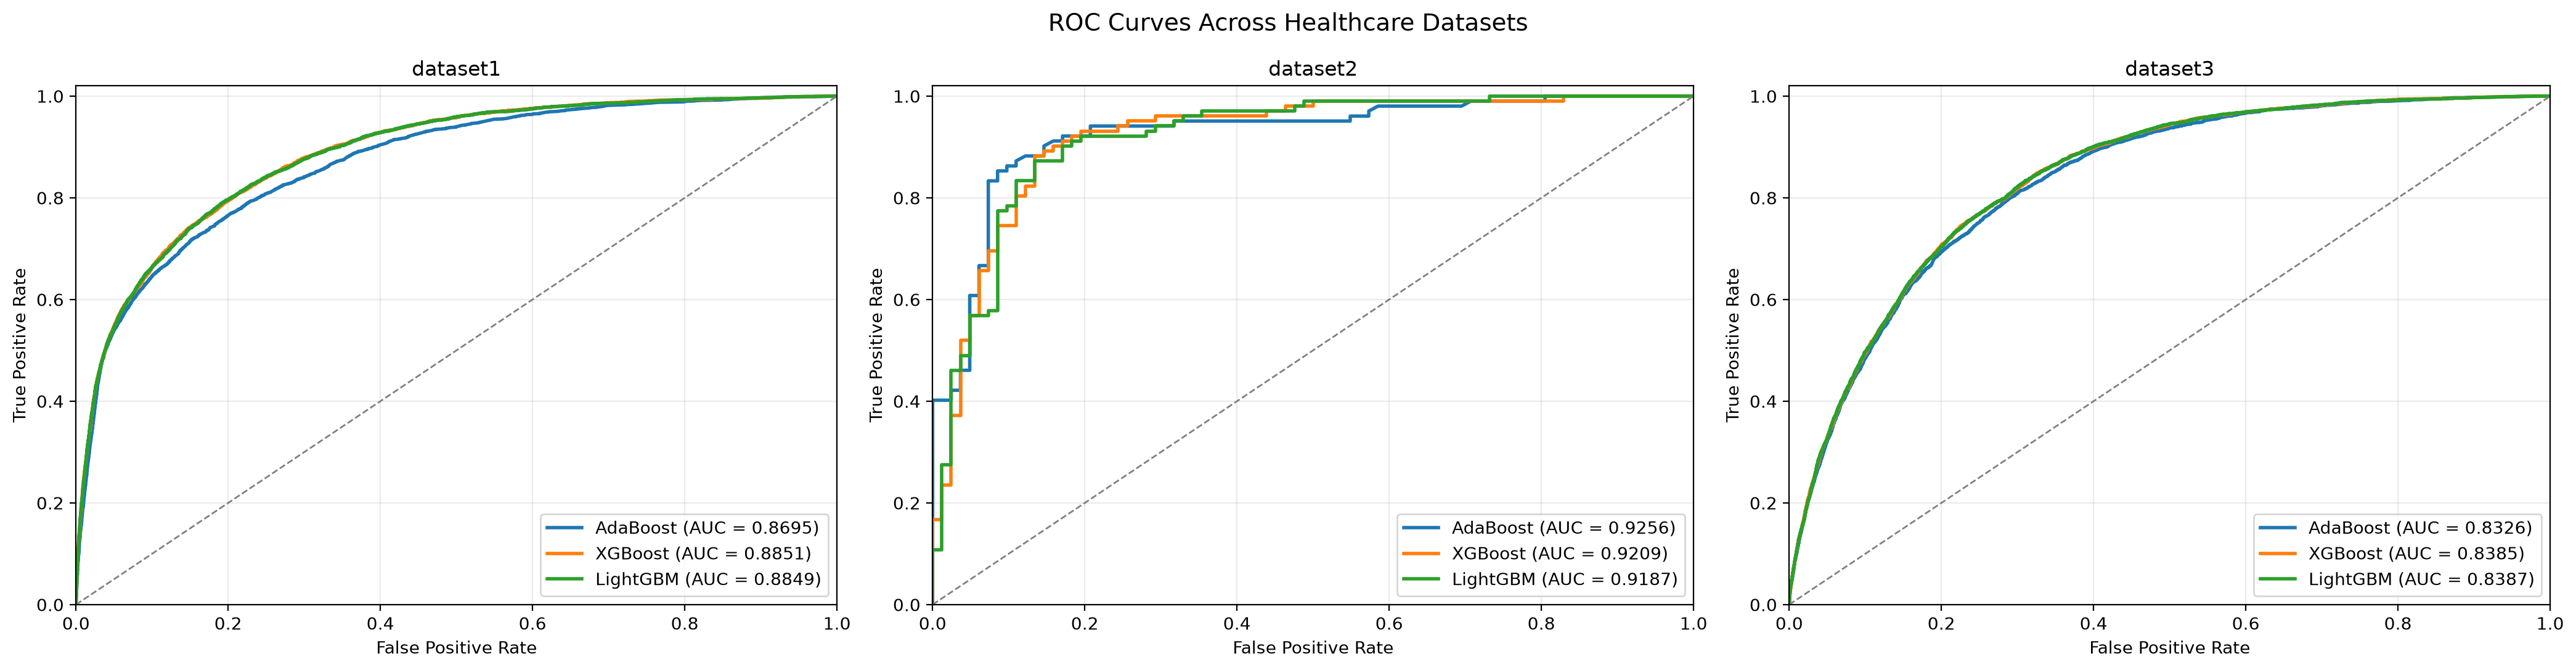
\includegraphics[width=0.95\linewidth]{Figures/roc_curves_all_datasets.png}
    \begin{minipage}{0.95\linewidth}
        \begin{figurecaptionmodern}
        \centering
        \capfig{ROC curves for the three models on the untouched hold-out test sets across the three healthcare datasets.}
        \label{fig:roc-all-datasets}
        \end{figurecaptionmodern}
    \end{minipage}
\end{figure}

The ROC visualization is consistent with the tabulated test results. The curves
are close on Dataset 1 and Dataset 3, where XGBoost and LightGBM provide similar
ranking performance. Dataset 2 has the highest test AUC values overall, but its
step-shaped curves also reflect the smaller test sample and therefore should not
be interpreted as evidence of uniformly better clinical performance across
datasets. The figure supports comparing ranking behavior within each dataset,
not pooling patients from different prediction tasks.

\begin{table}[H]
\centering
\begin{minipage}{0.90\linewidth}
\centering
    \refstepcounter{table}
    \begin{captionbelowboxaivn}
        \captable{Performance on the untouched hold-out test partitions after refitting on the full development data.}
        \label{tab:holdout_model_results}
    \end{captionbelowboxaivn}

        $\rho=0.9324$ but Kendall $\tau=0.7990$. Both values indicate positive and
    \small

    \begin{tabularx}{\linewidth}{@{}
        >{\raggedright\arraybackslash}X
        >{\raggedright\arraybackslash}X
        >{\centering\arraybackslash}X
        >{\centering\arraybackslash}X
        >{\centering\arraybackslash}X
        >{\centering\arraybackslash}X@{}}
\textbf{Dataset} & \textbf{Model} & \textbf{ROC-AUC} & \textbf{PR-AUC} & \textbf{Recall} & \textbf{F1} \\
\hline
Dataset 1 & AdaBoost & 0.8695 & 0.3860 & 0.6705 & 0.3657 \\
 & XGBoost & 0.8850 & 0.4169 & 0.7712 & 0.3255 \\
 & LightGBM & 0.8850 & 0.4187 & 0.7694 & 0.3259 \\
\hline
Dataset 2 & AdaBoost & 0.9256 & 0.9394 & 0.8529 & 0.8832 \\
 & XGBoost & 0.9224 & 0.9216 & 0.8333 & 0.8586 \\
 & LightGBM & 0.9189 & 0.9166 & 0.8431 & 0.8643 \\
\hline
Dataset 3 & AdaBoost & 0.8326 & 0.3672 & 0.7674 & 0.3788 \\
 & XGBoost & 0.8384 & 0.3756 & 0.7963 & 0.3773 \\
 & LightGBM & 0.8385 & 0.3763 & 0.7925 & 0.3789 \\
        \end{tabularx}
\end{minipage}
\end{table}

\subsection{Predictive Stability Across Cross-Validation Folds (RQ2)}

The fold-level results also reveal clear differences in stability across the
three datasets. Dataset 1 and Dataset 3 produced small standard deviations for
all three models. For example, XGBoost obtained ROC-AUC standard deviations of
0.0033 on Dataset 1 and 0.0027 on Dataset 3. LightGBM showed similarly small
variation, indicating that the two gradient-boosted models were not highly
sensitive to the particular fold assignment on the two larger datasets.

Dataset 2 exhibited noticeably greater fold-to-fold variation. Its development
partition contains only 734 samples, compared with 353,653 for Dataset 1 and
183,824 for Dataset 3. XGBoost ROC-AUC ranged from 0.8676 to 0.9465 across the
five folds, while AdaBoost ranged from 0.8547 to 0.9673 and LightGBM ranged from
0.8651 to 0.9497. The larger variability is therefore consistent with the
smaller sample size: each validation fold contains fewer observations, so the
composition of a single fold has a greater influence on the measured score.

The final hold-out results were generally close to the corresponding
cross-validation means. For example, Dataset 1 XGBoost achieved a mean CV
ROC-AUC of 0.8873 and a hold-out ROC-AUC of 0.8851, while Dataset 3 XGBoost
achieved 0.8386 in CV and 0.8385 on the hold-out set. This agreement provides
additional evidence that the reported cross-validation estimates are not driven
by a single unusually favorable split.

Overall, RQ2 is answered by finding that predictive performance is highly stable
on the two large datasets but less stable on the small Heart Failure Prediction
dataset. The pattern is observed across all three algorithms, suggesting that
dataset size and fold composition contribute more to the observed instability
than the choice among the three boosting methods alone.


\subsection{SHAP Feature-Importance Stability Across Cross-Validation Folds (RQ3)}
\label{subsec:shap_results}

Following the fold-wise explainability procedure described in
Section~\ref{subsec:shap_methodology}, RQ3 evaluates whether SHAP-based global
feature-importance rankings remain consistent when the training and validation
partitions change across cross-validation folds. For every dataset--model
combination, all ten unique pairs of the five folds are compared using Kendall's
$\tau$, Spearman's $\rho$, and top-10 Jaccard similarity.

Table~\ref{tab:shap_stability_results} shows that the SHAP feature rankings are
generally stable across folds for all nine dataset--model combinations.
Mean Spearman correlations range from 0.9324 to 0.9921, indicating strong
agreement in the complete feature ordering. Mean Kendall coefficients range
from 0.7990 to 0.9636, providing additional evidence that most pairwise feature
ordering relationships are preserved across folds. Top-10 Jaccard similarity
ranges from 0.7758 to 1.0000, indicating that the most influential feature sets
are also largely consistent.

\begin{table}[H]
\centering
\begin{minipage}{0.90\linewidth}
\centering
    \refstepcounter{table}
    \begin{captionbelowboxaivn}
        \captable{Mean SHAP feature-ranking stability across the ten pairwise comparisons of five cross-validation folds.}
        \label{tab:shap_stability_results}
    \end{captionbelowboxaivn}

    \renewcommand{\arraystretch}{1.1}
    \small

    \begin{tabularx}{\linewidth}{@{}
        >{\raggedright\arraybackslash}X
        >{\raggedright\arraybackslash}X
        >{\centering\arraybackslash}X
        >{\centering\arraybackslash}X
        >{\centering\arraybackslash}X@{}}
\textbf{Dataset} &
\textbf{Model} &
\textbf{Kendall $\tau$} &
\textbf{Spearman $\rho$} &
\textbf{Top-10 Jaccard} \\
\hline
Dataset 1 & AdaBoost & 0.9593 & 0.9644 & 0.9273 \\
          & XGBoost  & 0.7990 & 0.9324 & 0.8273 \\
          & LightGBM & 0.8057 & 0.9368 & 0.7758 \\
\hline
Dataset 2 & AdaBoost & 0.8536 & 0.9410 & 0.8061 \\
          & XGBoost  & 0.8118 & 0.9346 & 0.8545 \\
          & LightGBM & 0.8301 & 0.9422 & 0.8364 \\
\hline
Dataset 3 & AdaBoost & 0.9636 & 0.9921 & \textbf{1.0000} \\
          & XGBoost  & 0.9255 & 0.9814 & \textbf{1.0000} \\
          & LightGBM & 0.8996 & 0.9735 & 0.9273 \\
        \end{tabularx}
\end{minipage}
\end{table}

Dataset 3 demonstrates particularly strong explanation stability. AdaBoost and
XGBoost both obtain a mean top-10 Jaccard score of 1.0000, indicating that the
same set of ten most influential features is retained across every fold pair.
LightGBM achieves the highest overall mean Spearman correlation of 0.9735,
showing that its complete feature ranking is also highly consistent. The high
Kendall coefficients for all three models further confirm that the relative
ordering of feature pairs changes only modestly across partitions.

Dataset 1 also exhibits strong overall stability, although the different
metrics reveal some variation near the top of the ranking. AdaBoost achieves
the strongest agreement on this dataset, with mean Kendall $\tau=0.9593$,
Spearman $\rho=0.9644$, and top-10 Jaccard similarity of 0.9273. LightGBM,
however, obtains a high Spearman correlation of 0.9368 while its top-10 Jaccard
similarity is lower at 0.7758. This result indicates that the complete ranking
remains similar across folds even though several features near the top-10
boundary exchange positions or move into and out of the top feature set.

The difference between the Kendall and Spearman measurements is also
informative. For example, Dataset 1 XGBoost achieves Spearman
$\rho=0.9324$ but Kendall $\tau=0.7990$. Both values indicate positive and
strong ranking agreement, but Kendall's lower value suggests that some
pairwise feature orderings change across folds even though the overall ranking
structure remains similar. Reporting both statistics therefore provides a more
complete view of explanation robustness than relying on a single correlation
measure.

Dataset 2 remains reasonably stable despite being substantially smaller than
Datasets 1 and 3. All three models obtain mean Spearman correlations greater
than 0.93, while mean Kendall coefficients range from 0.8118 to 0.8536.
Top-10 Jaccard similarity ranges from 0.8061 to 0.8545. These values indicate
that the majority of important features remain consistently ranked even though
some movement occurs between folds.

The SHAP beeswarm plots complement the global importance rankings by showing
both the magnitude and direction of feature contributions. Features appearing
near the top of the beeswarm plots have large absolute effects on the model
output, while the horizontal distribution of SHAP values indicates whether
particular feature values tend to increase or decrease the predicted risk.
The corresponding mean absolute SHAP bar plots provide a simpler view of
global importance, and the violin plots show the distribution of SHAP effects
for the leading features.

The feature-ranking heatmaps provide a direct visualization of explanation
stability across folds. Features whose heatmap cells remain at similar rank
values across all five folds can be considered highly stable, whereas large
changes in rank indicate sensitivity to the particular training partition.
This visualization is especially useful for distinguishing small changes near
the top-10 cutoff that may reduce Jaccard similarity without substantially
changing the complete ranking.

The fold-correlation heatmaps provide an additional model-level view of
stability. High off-diagonal Spearman correlations indicate that different
training folds produce similar global feature orderings. A fold with
substantially lower correlations to the other folds would suggest that the
corresponding training partition produces a noticeably different explanation.
Together with the ranking heatmaps, these plots allow the numerical stability
scores to be visually inspected rather than interpreted only from aggregated
statistics.

Overall, RQ3 is answered by finding that SHAP-based global feature-importance
rankings are robust to cross-validation partitioning for the evaluated boosting
models. This conclusion is supported by three complementary measures:
Kendall's $\tau$ shows strong pairwise ordering agreement, Spearman's $\rho$
shows high consistency in complete feature rankings, and top-10 Jaccard
similarity shows that the most influential feature sets are generally
preserved.

At the same time, the results demonstrate why multiple stability metrics are
necessary. A model can maintain a high full-ranking correlation while still
showing changes in the membership of its top-10 features. Consequently,
explanation stability should not be judged from a single correlation
coefficient alone. Combining rank correlations, top-feature overlap,
feature-ranking heatmaps, and fold-correlation heatmaps provides a more
complete assessment of the reproducibility of model explanations.

The observed SHAP stability should be interpreted as evidence of explanation
robustness rather than causal validity. A feature that is consistently
important across folds is repeatedly used by the model under the observed data
distribution, but this does not imply that changing that feature would
causally alter a patient's health outcome. In addition, because AdaBoost uses
permutation SHAP while XGBoost and LightGBM use TreeSHAP, raw SHAP magnitudes
are not used for direct cross-model comparisons. RQ3 therefore focuses on
within-model fold-to-fold ranking stability, which remains comparable across
the experimental protocol.

\begin{figure}[H]
    \centering
    \begin{minipage}{0.32\linewidth}
        \centering
        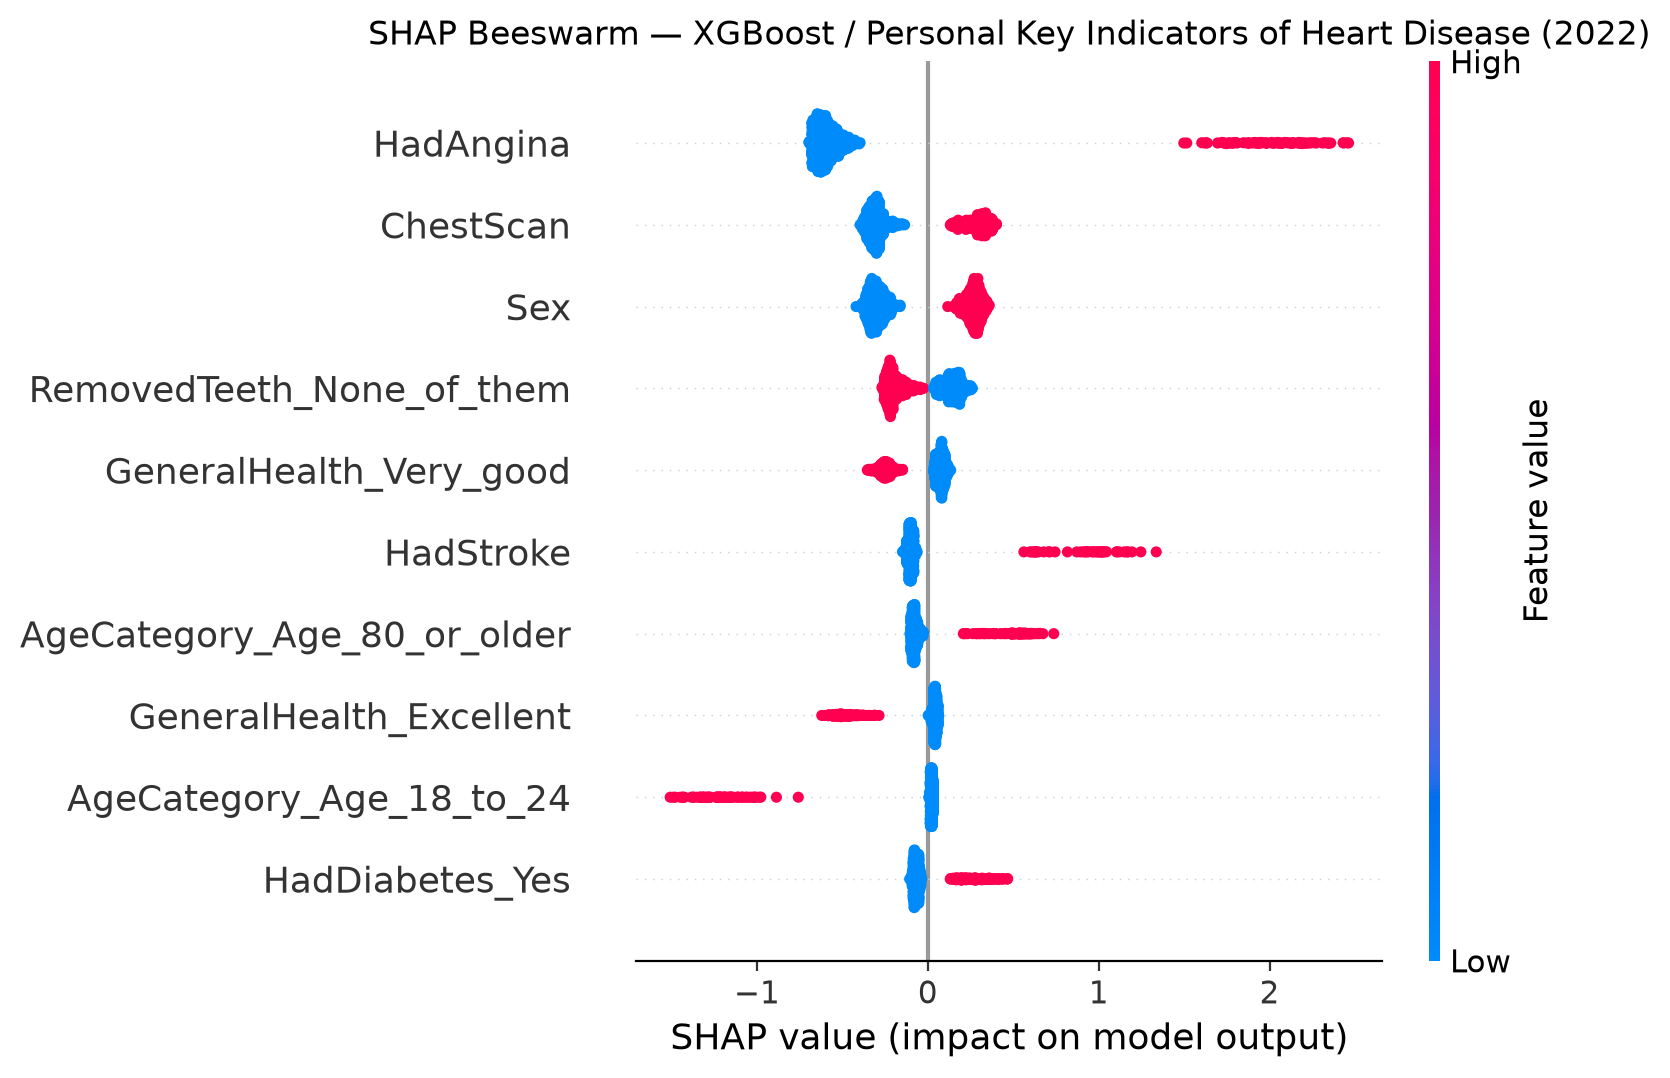
\includegraphics[width=\linewidth]{Figures/dataset1_xgboost_beeswarm.png}
    \end{minipage}\hfill
    \begin{minipage}{0.32\linewidth}
        \centering
        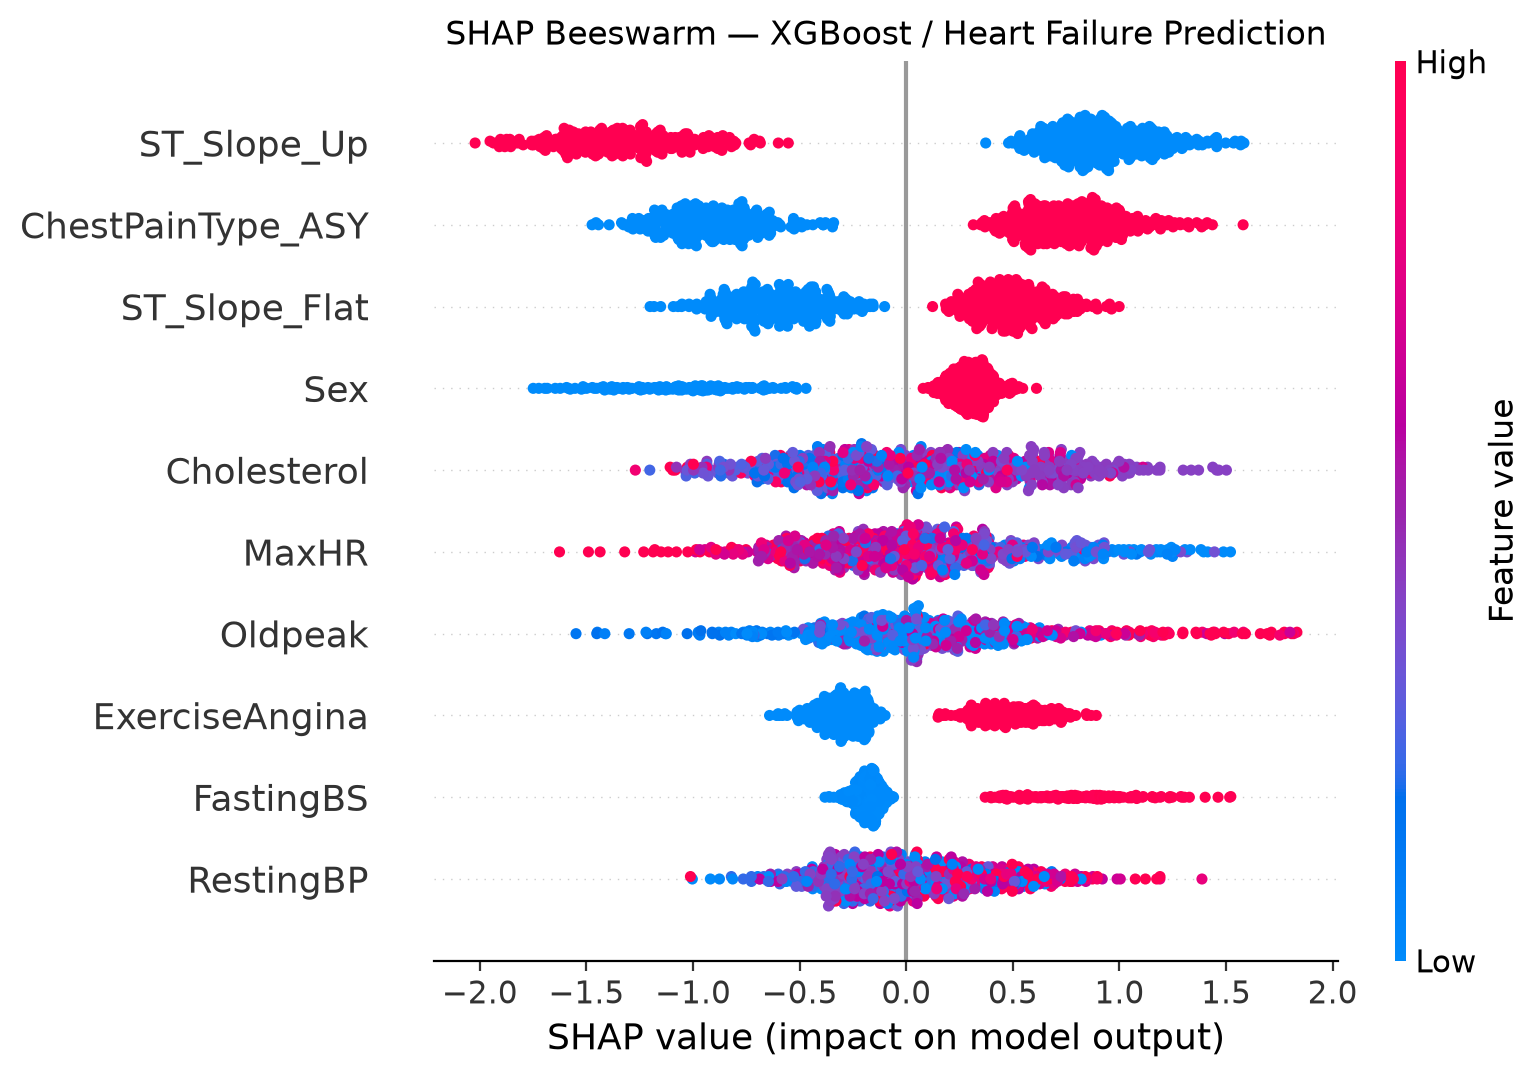
\includegraphics[width=\linewidth]{Figures/dataset2_xgboost_beeswarm.png}
    \end{minipage}\hfill
    \begin{minipage}{0.32\linewidth}
        \centering
        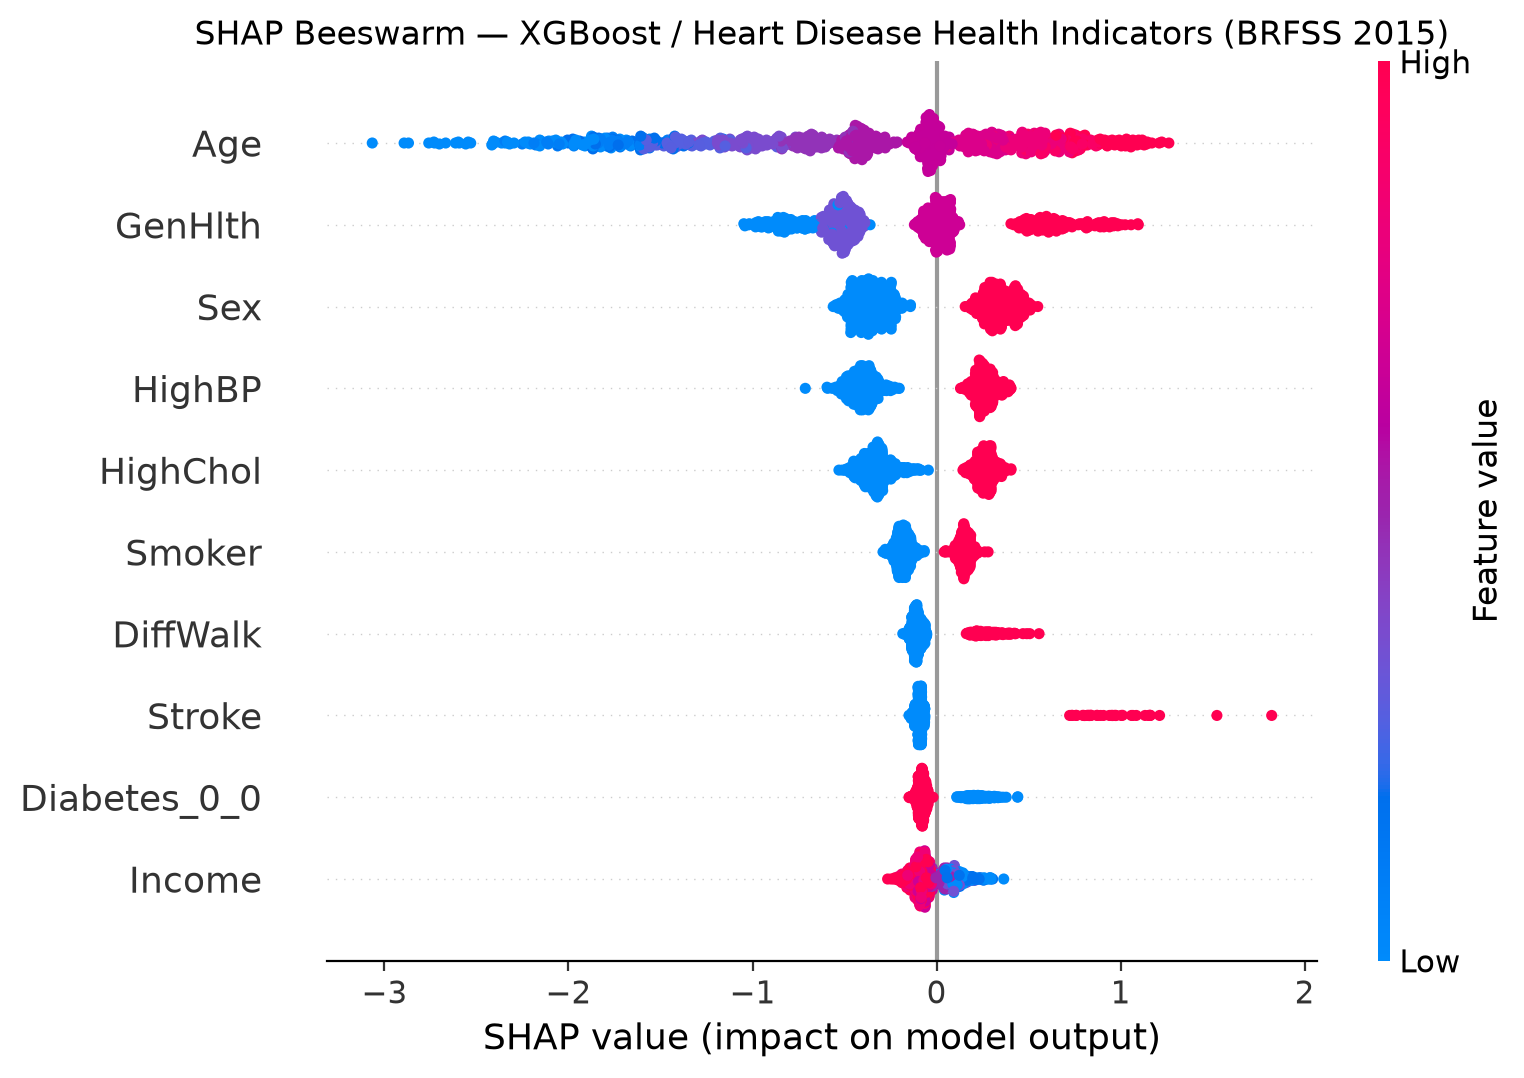
\includegraphics[width=\linewidth]{Figures/dataset3_xgboost_beeswarm.png}
    \end{minipage}
    \begin{minipage}{0.95\linewidth}
        \begin{figurecaptionmodern}
        \centering
        \capfig{SHAP beeswarm plots for XGBoost on Dataset 1, Dataset 2, and Dataset 3, respectively.}
        \label{fig:xgboost-beeswarm-datasets}
        \end{figurecaptionmodern}
    \end{minipage}
\end{figure}

The beeswarm plots show that the most influential features are dataset-specific.
For Dataset 1, \texttt{HadAngina}, \texttt{ChestScan}, and \texttt{Sex} occupy
the leading positions. Dataset 2 is dominated by \texttt{ST\_Slope\_Up},
\texttt{ChestPainType\_ASY}, and \texttt{ST\_Slope\_Flat}, whereas Dataset 3
is led by \texttt{Age}, \texttt{GenHlth}, and \texttt{Sex}. The horizontal
position indicates contribution direction and magnitude, while color encodes
the feature value. These patterns show why a single cross-dataset feature
interpretation would be misleading even when the same model family is used.

\begin{figure}[H]
    \centering
    \begin{minipage}{0.48\linewidth}
        \centering
        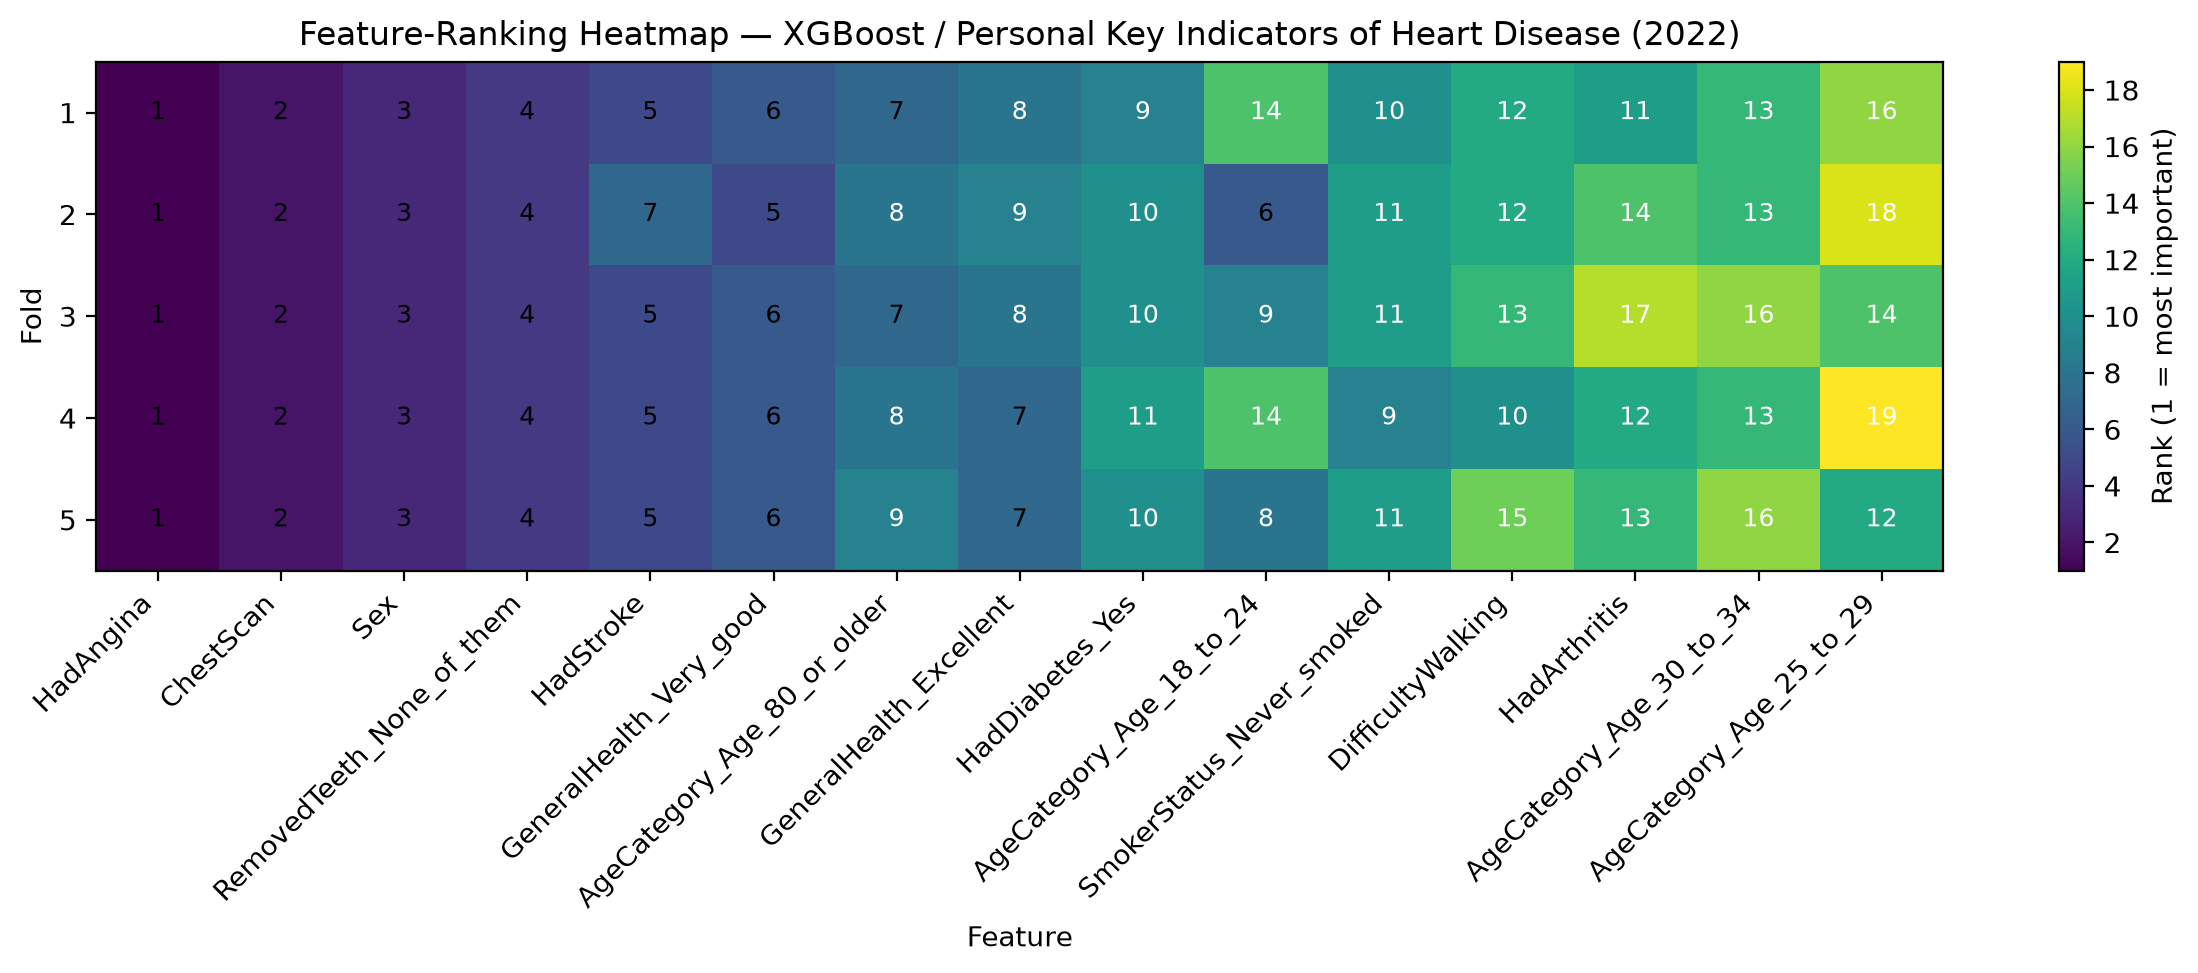
\includegraphics[width=\linewidth]{Figures/dataset1_xgboost_ranking_heatmap.png}
    \end{minipage}\hfill
    \begin{minipage}{0.48\linewidth}
        \centering
        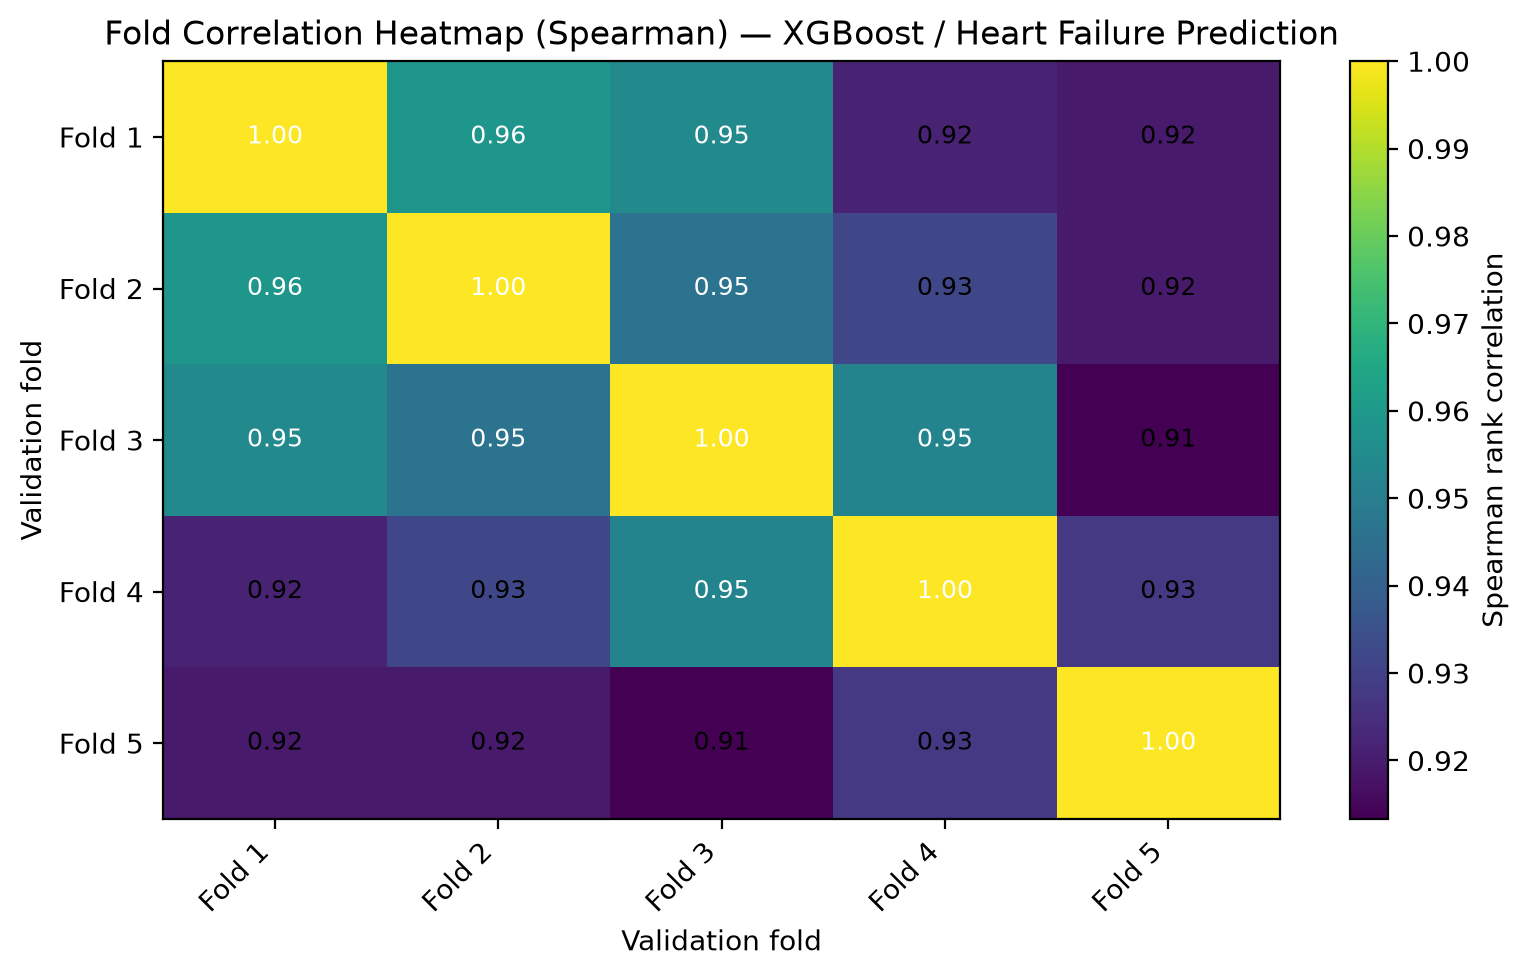
\includegraphics[width=\linewidth]{Figures/dataset2_xgboost_fold_correlation_heatmap.png}
    \end{minipage}
    \begin{minipage}{0.95\linewidth}
        \begin{figurecaptionmodern}
        \centering
        \capfig{Representative SHAP stability visualizations: feature-ranking heatmap for Dataset 1 and fold-correlation heatmap for Dataset 2 using XGBoost.}
        \label{fig:shap-stability-visualizations}
        \end{figurecaptionmodern}
    \end{minipage}
\end{figure}

The ranking heatmap makes the fold-level movement of individual features
visible, while the correlation heatmap summarizes agreement between complete
rankings. The high off-diagonal correlations in the Dataset 2 example are
consistent with its mean Spearman value of 0.9346, even though its smaller
sample produces larger predictive variability. Together, the plots clarify
that explanation stability concerns reproducibility of model rankings, not
causal importance or clinical validity.



\subsection{Discussion}

Taken together, the three research questions provide complementary evidence
about predictive quality and interpretability. RQ1 shows that XGBoost provides
the strongest overall predictive ranking across the three datasets, with
LightGBM very close on ROC-AUC and PR-AUC and AdaBoost retaining the highest
cross-dataset mean F1. RQ2 shows that predictive scores are highly stable on the
two large datasets but vary more on the smaller Heart Failure Prediction
dataset. RQ3 extends the stability analysis from prediction metrics to model
explanations and finds that the SHAP feature rankings remain highly consistent
across folds for all three boosting methods.

The SHAP results should be interpreted as measures of explanation stability,
not as evidence of causality. A feature can be consistently important to a
model because it is predictive under the observed data distribution, but this
does not establish that changing the feature would causally change a patient's
risk. In addition, raw SHAP magnitudes are not compared directly between
AdaBoost and the two gradient-boosted models because AdaBoost is explained with
permutation SHAP whereas XGBoost and LightGBM use TreeSHAP. The study therefore
bases RQ3 on within-model fold-to-fold ranking consistency, which is comparable
across the experimental protocol.

Overall, the combined findings indicate that the strongest models are not only
competitive in predictive performance but also produce feature-importance
patterns that are reproducible across data partitions. This is useful for
healthcare risk-prediction studies because an explanation that changes sharply
with a different fold would be difficult to trust even if average predictive
performance were high. The observed stability therefore provides an additional
criterion, alongside ROC-AUC, PR-AUC, Recall, and F1, for assessing the
robustness of the evaluated models.



% -----------------------------------------------------------------------
% Section commented out per team request (2026-08-05): the required report
% structure (see the mucluc/TOC image supplied by the team) has no separate
% Error Analysis and Limitations section. Kept in source, not rendered.
% -----------------------------------------------------------------------
\iffalse
\fi

% -----------------------------------------------------------------------
% Section commented out per team request (2026-08-05): the required report
% structure has no separate Replicate the Results section. The repository
% link, structure, and reproduction commands are kept in the Appendix
% instead. Kept in source, not rendered.
% -----------------------------------------------------------------------
\iffalse
\newpage
\fi

\section{Conclusion and Future Work}
\label{sec:conclusion_future_work}

\subsection{Conclusion}

\newpage
\section{References}
\label{section:references}
\nocite{*}
\vspace{-3.2em}
\printbibliography

\newpage
\begin{appendices}
\begin{enumerate}
\item \textbf{AIVIETNAM:} Further information about AIVIETNAM can be found \href{https://aivietnam.edu.vn/}{here}.
\item \textbf{GitHub Repository:}
\item \textbf{Dataset:}
\item \textbf{Demo Video / Presentation:}
\begin{itemize}
    \item Link demo video: \href{https://youtu.be/a0pVMnRgGaE}{Link demo}
    \item Link slide presentation: \href{https://drive.google.com/file/d/1foDtkD4MwgivJIOTfOiVh2aazJ1p3nHq/view?usp=sharing}{Link slide presentation}
\end{itemize}
\end{enumerate}
\end{appendices}

\end{document}
